\documentclass[a4paper]{article}
\usepackage{fullpage}
\usepackage{mathptmx}
\newcommand{\mse}[0]{\texttt{monitored-session-erlang}}
\usepackage{url}
\usepackage{parskip}
\usepackage[scaled=0.7]{beramono}
\usepackage[numbers]{natbib}
\usepackage{graphicx}
\usepackage{listings}
\usepackage{float}
\usepackage{listings}
\usepackage{upquote}
\usepackage{color}

\definecolor{bluekeywords}{rgb}{0.13,0.13,1}
\definecolor{greencomments}{rgb}{0,0.5,0}
\definecolor{turqusnumbers}{rgb}{0.17,0.57,0.69}
\definecolor{redstrings}{rgb}{0.5,0,0}

\lstdefinelanguage{Scribble}{
  morekeywords={
  	global, protocol, role, from, to, interruptible, with, do, instantiates, par, and, rec, continue, choice, at, initiates, handle, returning, call, local, or
  },
  otherkeywords={ },
  keywordstyle=\color{bluekeywords},
  sensitive=true,
  %basicstyle=\scriptsize\ttfamily,
  basicstyle=\linespread{0.9}\ttfamily,
	breaklines=true,
  xleftmargin=\parindent,
  belowskip=\bigskipamount,
  aboveskip=\bigskipamount,
  tabsize=4,
  morecomment=[l][\color{greencomments}]{///},
  morecomment=[l][\color{greencomments}]{//},
  morecomment=[s][\color{greencomments}]{{(*}{*)}},
  morestring=[b]",
  showstringspaces=false,
  literate={`}{\`}1,
  frame=none,
  showlines=false,
  frame=single,
  stringstyle=\color{redstrings},
}

\lstset{
  language=Scribble,
  showstringspaces=false,
  formfeed=\newpage,
  tabsize=2,
  commentstyle=\itshape,
  basicstyle=\linespread{0.9}\ttfamily,
  %captionpos=b,
  %belowcaptionskip=4pt,
}
% \renewcommand*\familydefault{\ttdefault} %% Only if the base font of the document is to be typewriter style
\usepackage[T1]{fontenc}

\title{Erlang DNS Server}
\author{Simon Fowler}
\begin{document}
\maketitle

\section{Introduction}
In this report, we describe the adaptation of a freely-available DNS server, \texttt{erlang-dns}\footnote{\url{http://www.github.com/hcvst/erlang-dns}} to use multiparty session types, within the \mse{}~\cite{fowler:msc} framework for monitoring session-typed Erlang applications.

The actor model~\cite{agha:actors,hewitt:actors}, while originally developed in the context of a model for artificial intelligence, has found much use in developing scalable and fault-tolerant distributed systems. Erlang~\cite{armstrong:erlang} is a programming language, which, following the actor model, disallows communication via shared memory, instead requiring all co-ordination to happen via explicit message passing. 

The \texttt{erlang-dns} application a server for the Domain Name System (DNS)~\cite{rfc1035,rfc2535} which allows domain names to be resolved to IP addresses.
Unlike the Simple Mail Transfer Protocol (SMTP) use case, the DNS protocol is a simple request-response protocol: instead, the request is encoded using a sophisticated packet structure with many inter-dependencies: as an aside, these are possible to encode using dependent types~\cite{fowler:bsc}. The purpose of this report, however, is to show how multiparty session types can be used to describe nontrivial communication patterns \emph{within the DNS server itself}.

\section{Description}
The \texttt{erlang-dns} project is an open-source Erlang DNS server. The Erlang supervision tree for \texttt{erlang-dns} is shown in Figure~\ref{edns-supervision-tree}.

In particular, there are three types of actors that are of interest:

\begin{itemize}
\item \texttt{ed\_udp\_handler} (denoted by \texttt{Req$_0$} ... \texttt{Req$_n$}): these actors handle incoming UDP requests.
\item \texttt{ed\_zone\_data\_server} (denoted by \texttt{.com}, \texttt{.net}): these actors contain mappings from domain names to IP addresses, for each type of 
\item \texttt{ed\_zone\_registry\_server}: maps domain names to the actor \texttt{ed\_zone\_data\_server} PIDs.
\end{itemize}

At a high level, the steps taken upon receiving an incoming DNS request are as follows:

\begin{enumerate}
\item A \texttt{ed\_udp\_handler} actor is created to handle the DNS request
\item The \texttt{ed\_udp\_handler} decodes the request, and contacts the \texttt{ed\_zone\_registry\_server} with the requested domain name
\item The \texttt{ed\_zone\_registry\_server} attempts to find the actor responsible for the given domain name: if the domain name exists, then the PID of the \texttt{ed\_zone\_data\_server} is returned, whereas if the domain name does not exist, then an error is returned.
\item If the zone does not exist, and error packet response is sent to the client. If the zone \emph{does} exist, then the request is sent to the \texttt{ed\_zone\_data\_server}.
\item The \texttt{ed\_zone\_data\_server} responds with the relevant mapping entries.
\item The \texttt{ed\_udp\_handler} uses the response to either fulfil the request, sending a successful response to the client, or uses the response to make recursive queries.
\end{enumerate}

\begin{figure}
\centering
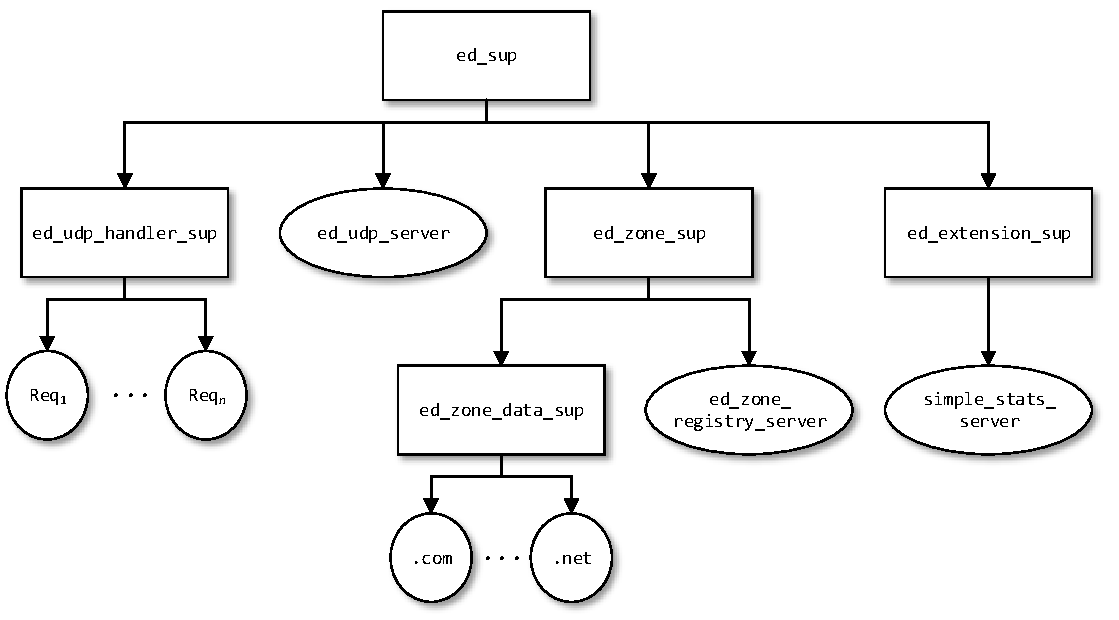
\includegraphics[width=0.7\textwidth]{Erlang-DNS-Tree.pdf}
\label{edns-supervision-tree}
\caption{Supervision Tree for \texttt{erlang-dns}}
\end{figure}

\section{Scribble Protocol}
We describe the multiparty session type using an extension of the Scribble~\cite{honda:scribble,scribblespec} protocol description language. Note that in order to encode the dynamic introduction of a new party into the session, we make use of \emph{subsessions}~\cite{demangeon:subsessions} to invite external participants. 
It is not possible to encode the protocol without subsessions, since the inhabitant of the \texttt{DNSZoneDataServer} role (the actor containing the mapping table for a particular DNS zone) is not known at the start of the protocol.
We also make use of a new construct \texttt{call} for encoding synchronous calls.

\begin{minipage}{\linewidth}
\begin{lstlisting}[language=scribble]
module src.com.simonjf.ScribbleExamples.DNSServer.DNSServer;

type <erlang> "atom" from "" as EncodedRequest;
type <erlang> "pid" from "" as ZonePID;
type <erlang> "atom" from "" as RRTree;
type <erlang> "string" from "" as DomainName;
type <erlang> "list" from "" as StringList;
type <erlang> "string" from "" as Zone;


global protocol HandleDNSRequest(role UDPHandlerServer, role DNSZoneRegServer) {
  rec QueryResolution {
    // Request the nearest zone
    FindNearestZone(DomainName) from UDPHandlerServer to DNSZoneRegServer;

    // Either we have it, or we don't...
    choice at DNSZoneRegServer {
        // If we do, then get the PID for the zone data server
        ZoneResponse(ZonePID) from DNSZoneRegServer to UDPHandlerServer;
        // Introduce the zone data server using a subsession
        UDPHandlerServer initiates GetZoneData(UDPHandlerServer, new DNSZoneDataServer) {
          // Now we've done that, we can do possible recursive lookups
          continue QueryResolution;
        }
    } or {
      InvalidZone() from DNSZoneRegServer to UDPHandlerServer;
    }
  }
}

global protocol GetZoneData(role UDPHandlerServer, role DNSZoneDataServer) {
    call ZoneDataRequest() returning RRTree from UDPHandlerServer to DNSZoneDataServer {}
}
\end{lstlisting}
\end{minipage}

The Scribble protocol consists of two separate protocols: \texttt{HandleDNSRequest}, which is the top-level protocol which co-ordinates how a request is handled, and \texttt{GetZoneData}, which requests the concrete zone data from the external participant.

There are three types of role:

\begin{itemize}
\item \texttt{UDPHandlerServer}: an actor spawned to handle a DNS request.
\item \texttt{DNSZoneRegServer}: an actor which acts as a registry for each individual DNS zone, mapping top-level DNS zone names to actor PIDs
\item \texttt{DNSZoneDataServer}: an actor which contains the zone data for each individual DNS zone
\end{itemize}

The first message is sent from the UDPHandlerServer to the DNSZoneRegServer to find the PID of the nearest zone. If this is not found, then the DNSZoneRegServer responds with an \texttt{InvalidZone()} message. If it is found, however, then the \texttt{DNSZoneRegServer} sends a \texttt{ZoneResponse} message, along with the PID of the actor holding the zone data. The \texttt{UDPHandlerServer} then initiates the \texttt{GetZoneData} subsession, directly inviting the returned PID to fulfil the \texttt{DNSZoneDataServer} role. Finally, the zone data is returned: the \texttt{UDPHandlerServer} is then free to make a recursive lookup if necessary.

\subsection{Local Projections}
\subsubsection{UDPHandlerServer}
\begin{minipage}{\textwidth}
\begin{lstlisting}[language=scribble]
module src.com.simonjf.ScribbleExamples.DNSServer.DNSServer_UDPHandlerServer;

type <erlang> "atom" from "" as EncodedRequest;
type <erlang> "pid" from "" as ZonePID;
type <erlang> "atom" from "" as RRTree;
type <erlang> "string" from "" as DomainName;
type <erlang> "list" from "" as StringList;
type <erlang> "string" from "" as Zone;

local protocol HandleDNSRequest at UDPHandlerServer(role UDPHandlerServer,role DNSZoneRegServer) {
  rec QueryResolution {
    FindNearestZone(DomainName) to DNSZoneRegServer;
    choice at DNSZoneRegServer {
      ZoneResponse(ZonePID) from DNSZoneRegServer;
      UDPHandlerServer initiates GetZoneData( UDPHandlerServer , new DNSZoneDataServer ) {
        continue QueryResolution;
      }
    } or {
      InvalidZone() from DNSZoneRegServer;
    }
  }
}

local protocol GetZoneData at UDPHandlerServer(role UDPHandlerServer,role DNSZoneDataServer) {
  send_call_request ZoneDataRequest() to DNSZoneDataServer;
  receive_call_response ZoneDataRequest(RRTree) from DNSZoneDataServer;
}
\end{lstlisting}
\end{minipage}

\subsubsection{DNSZoneRegServer}
\begin{minipage}{\textwidth}
\begin{lstlisting}[language=scribble]
module src.com.simonjf.ScribbleExamples.DNSServer.DNSServer_DNSZoneRegServer;

type <erlang> "atom" from "" as EncodedRequest;
type <erlang> "pid" from "" as ZonePID;
type <erlang> "atom" from "" as RRTree;
type <erlang> "string" from "" as DomainName;
type <erlang> "list" from "" as StringList;
type <erlang> "string" from "" as Zone;

local protocol HandleDNSRequest at DNSZoneRegServer(role UDPHandlerServer,role DNSZoneRegServer) {
  rec QueryResolution {
    FindNearestZone(DomainName) from UDPHandlerServer;
    choice at DNSZoneRegServer {
      ZoneResponse(ZonePID) to UDPHandlerServer;
    } or {
      InvalidZone() to UDPHandlerServer;
    }
  }
}
\end{lstlisting}
\end{minipage}

\subsubsection{DNSZoneDataServer}
\begin{minipage}{\textwidth}
\begin{lstlisting}[language=scribble]
module src.com.simonjf.ScribbleExamples.DNSServer.DNSServer_DNSZoneDataServer;

type <erlang> "atom" from "" as EncodedRequest;
type <erlang> "pid" from "" as ZonePID;
type <erlang> "atom" from "" as RRTree;
type <erlang> "string" from "" as DomainName;
type <erlang> "list" from "" as StringList;
type <erlang> "string" from "" as Zone;

local protocol GetZoneData at DNSZoneDataServer(role UDPHandlerServer,role DNSZoneDataServer) {
  receive_call_request ZoneDataRequest() from UDPHandlerServer;
  send_call_response ZoneDataRequest(RRTree) to UDPHandlerServer;
}
\end{lstlisting}
\end{minipage}

\section{Implementation using \mse{}}
The \mse{} framework is a framework for allowing actors in Erlang programs to be verified using multiparty session types. The system is described in depth elsewhere~\cite{fowler:msc}, but for the purposes of this document it sufficies to know that \mse{} provides a mechanism, based heavily on the work of~\cite{neykova:actors}, by which actors are \emph{invited} into a session.

The first step is to define a configuration file, which describes the roles that actors may play in each protocol.

\begin{lstlisting}[language=erlang]
-module(edns_conversation_conf).
-export([config/0]).

config() ->
  [{ed_zone_data_server, [{"GetZoneData", ["DNSZoneDataServer"]}]},
   {ed_zone_registry_server, [{"HandleDNSRequest", ["DNSZoneRegServer"]}]},
   {ed_udp_handler_server,
    [{"HandleDNSRequest", ["UDPHandlerServer"]},
     {"GetZoneData", ["UDPHandlerServer"]}]
   }].
\end{lstlisting}

This configuration file states, for example, that the \texttt{ed\_udp\_handler\_server} actor can play the ``\texttt{UDPHandlerServer}'' role in the ``\texttt{HandleDNSRequest}'' and ``\texttt{GetZoneData}'' protocols.

Next, each actor is implemented as an instance of the \texttt{ssa\_gen\_server} behaviour, which extends the Erlang \texttt{gen\_server} behaviour with monitoring capabilities. Each instance of the \texttt{ssa\_gen\_server} behaviour must provide the following callbacks:

\begin{itemize}
\item \texttt{ssactor\_init}: called when the actor is spawned
\item \texttt{ssactor\_join}: called when the actor is invited to fulfil a role in a protocol
\item \texttt{ssactor\_conversation\_established}: called when a session is established
\item \texttt{ssactor\_conversation\_error}: called if it is not possible to establish a session after inviting the actor
\end{itemize}

Each process is associated with an external monitoring process which maps the current protocol / role / session tuple with a finite state machine to monitor incoming and outgoing communication. A monitored message is only delivered if it is accepted by the FSM.

As an example, the \texttt{ed\_zone\_registry\_server} provides the following callbacks:

\begin{lstlisting}[language=erlang]
ssactor_init([], _MonitorPID) ->
  {0, gb_trees:empty()}.
ssactor_join(_, _, _, State) -> {accept, State}.
ssactor_conversation_established(_PN, _RN, _CID, _ConvKey, State) -> {ok, State}.
ssactor_conversation_error(_, _, _, State) -> {ok, State}.

ssactor_handle_message("HandleDNSRequest", "DNSZoneRegServer", _CID, _Sender,
                       "FindNearestZone", [DomainName], State, ConvKey) ->
  {NumRequests, GBTree} = State,
  NameTails = ed_utils:tails(string:tokens(DomainName, ".")),
  Names = lists:map(fun(X) -> string:join(X, ".") end, NameTails),
  IsZoneNotDefined = fun(Z) -> not gb_trees:is_defined(Z, GBTree) end,
  case lists:dropwhile(IsZoneNotDefined, Names) of
    [] ->
      conversation:send(ConvKey, ["UDPHandlerServer"], "InvalidZone", [], []);
    [H|_] ->
      Pid = gb_trees:get(H, GBTree),
      conversation:send(ConvKey, ["UDPHandlerServer"], "ZoneResponse", ["ZonePID"], [Pid])
  end,
  {ok, {NumRequests + 1, GBTree}}.
\end{lstlisting}

Here, we see that the actor will always accept an invitation. The \texttt{ssactor\_handle\_message} is called upon receipt of a monitored asynchronous message, providing the current protocol name, role name, session ID, sender, message name, payload, actor state, and session key (\texttt{ConvKey}). The session key is an opaque value containing information about the current protocol, role, and session key: this is required to dispatch outgoing messages to the correct monitor.
In order to send a monitored asynchronous message, the \texttt{conversation:send} function is used. This takes the session key, list of roles, message name, message payload types, and payload.

To start a new subsession, the \texttt{conversation:subsession} function is used. This takes the current session key; the name of the protocol that should be started; a list of \emph{internal invitations} (that is, roles which should be populated using the inhabitants from the current session) and \emph{external invitations}, which specify role-PID mappings for actors which are not part of the current session.

\begin{lstlisting}
get_zone(Pid, ConvKey) ->
  conversation:start_subsession(ConvKey, "GetZoneData", ["UDPHandlerServer"],
                                [{"DNSZoneDataServer", Pid}]).
\end{lstlisting}



\section{FSMs}
\subsection{UDPHandlerServer}
\begin{figure}[H]
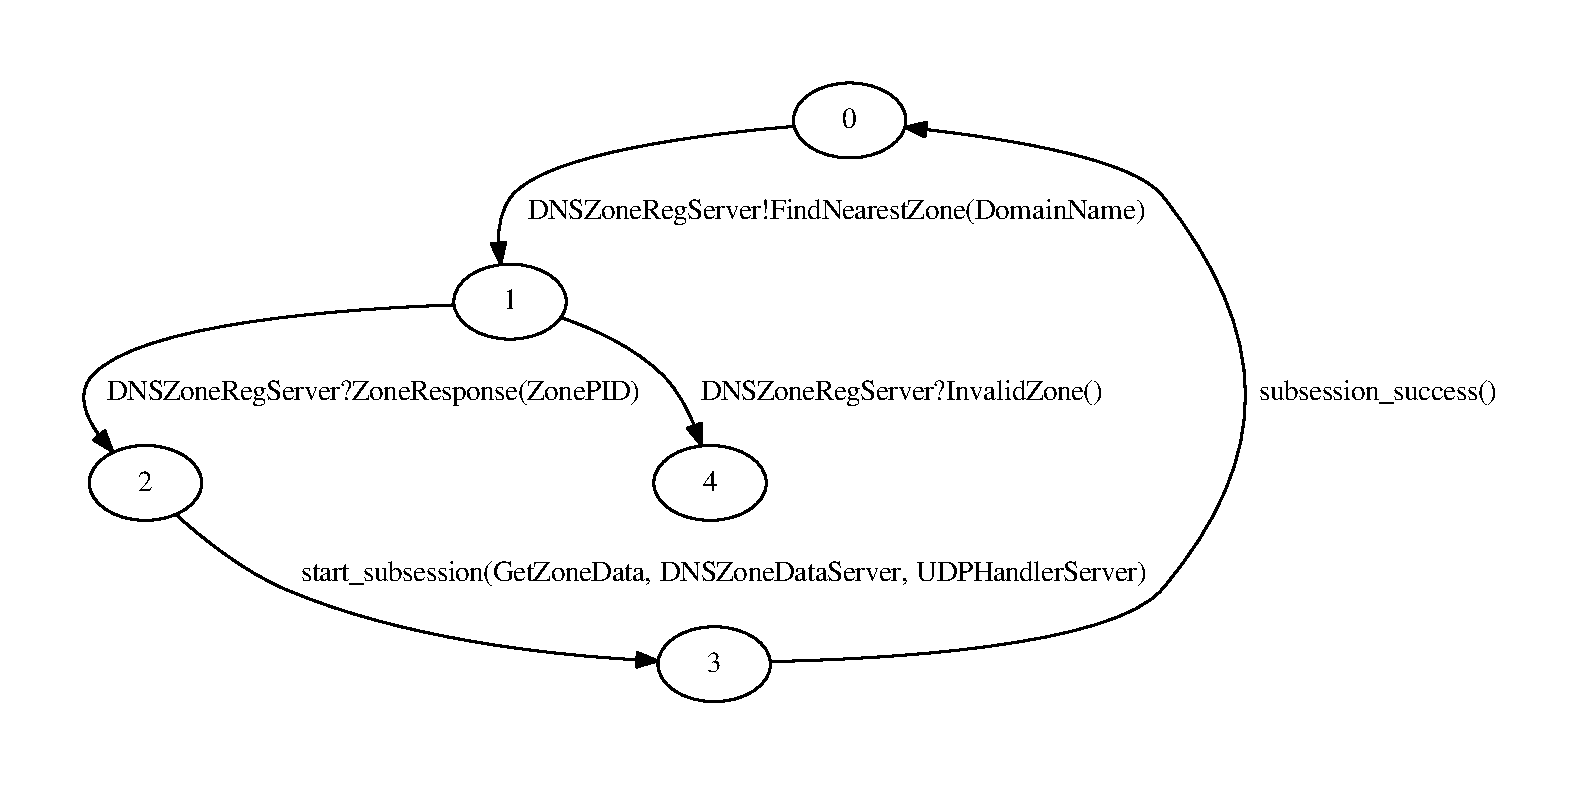
\includegraphics[width=0.6\textwidth]{handledns_udphandlerserver_dot.pdf}
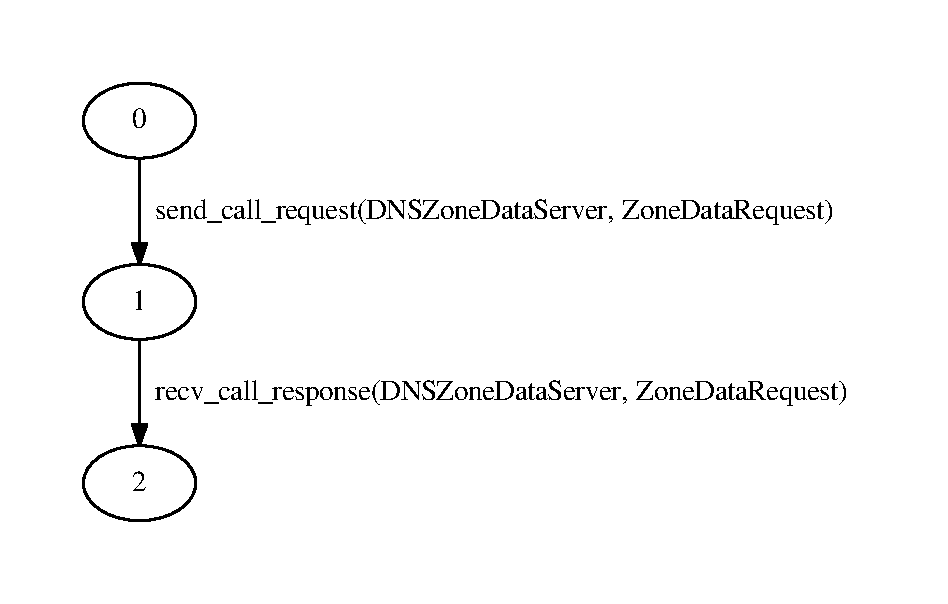
\includegraphics[width=0.4\textwidth]{getzonedata_udphandlerserver_dot.pdf}
\label{fsm-udphandlerserver}
\caption{Monitor FSMs for \texttt{UDPHandlerServer} in \texttt{HandleDNSRequest} and \texttt{GetZoneData}}
\end{figure}

\subsection{DNSZoneRegServer}
\begin{figure}[H]
\centering
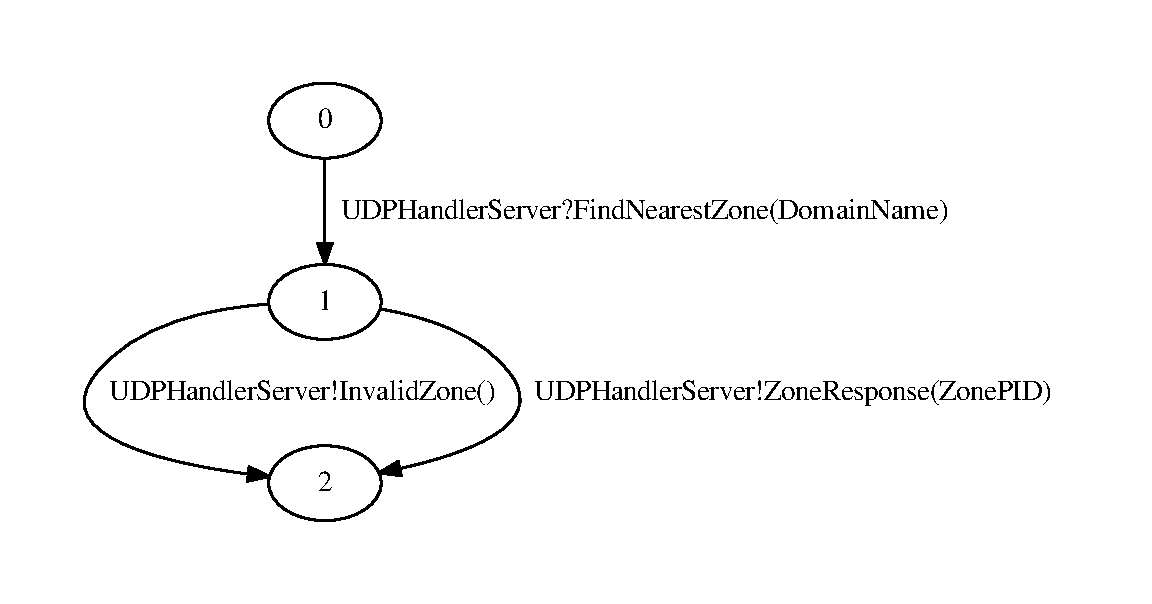
\includegraphics[width=0.4\textwidth]{handledns_zoneregserver_dot.pdf}
\label{fsm-zoneregserver}
\caption{Monitor FSMs for \texttt{DNSZoneRegServer} in \texttt{HandleDNSRequest}}
\end{figure}

\subsection{DNSZoneDataServer}
\begin{figure}[H]
\centering
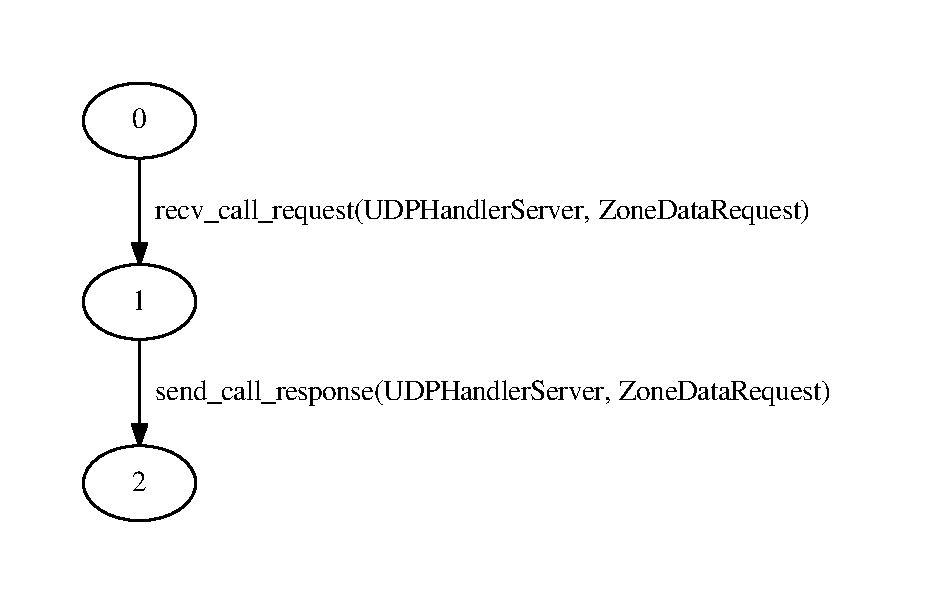
\includegraphics[width=0.6\textwidth]{getzonedata_zonedataserver_dot.pdf}
\label{fsm-zonedataserver}
\caption{Monitor FSMs for \texttt{DNSZoneRegServer} in \texttt{GetZoneData}}
\end{figure}


\section{Sequence Diagram}

\begin{figure}[H]
\centering
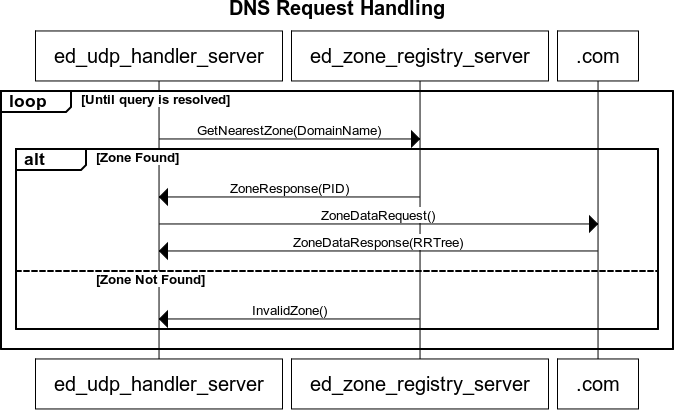
\includegraphics[width=0.7\textwidth]{DNSServer-Messages.png}
\end{figure}

\bibliographystyle{plainnat}
\bibliography{simonfowler}
\end{document}